\section{Architectural Design}

\subsection{Overview: high-level components and interactions}

\begin{figure}[H]
    \centering
    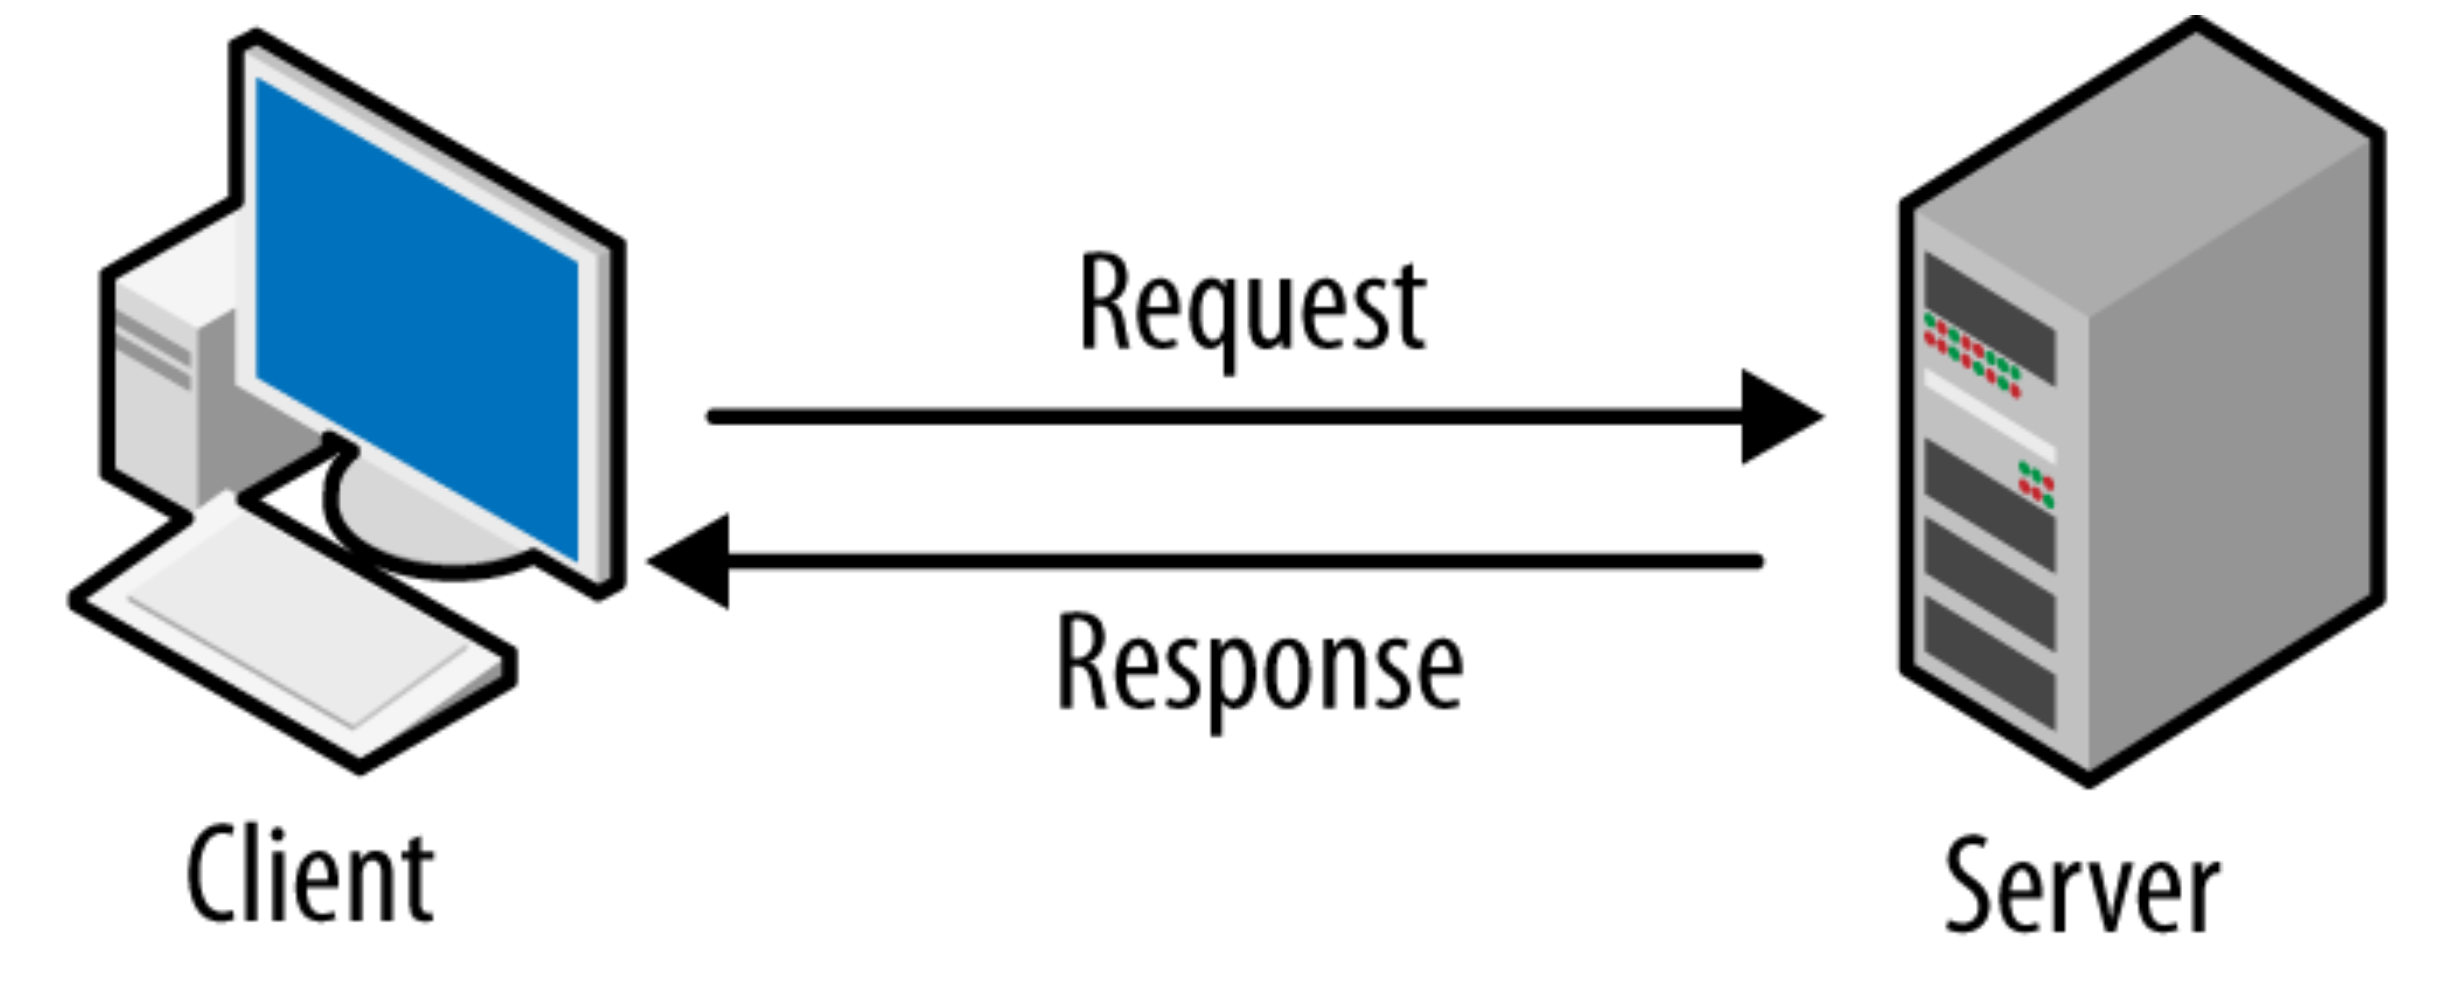
\includegraphics[width=0.6\textwidth]{DD/img/section2/client-server-1.png} 
    \caption{Client-Server paradigm}
    \label{fig:client_server}
\end{figure}

The \textit{Best Bike Paths} (BBP) system is designed as a distributed application adhering to the \textbf{Client-Server paradigm} (represented in Figure \ref{fig:client_server}). The architecture is engineered to support two primary user categories: \textit{Registered Users}, who actively contribute data through trip recordings and reports, and \textit{Unregistered Users}, who utilize the system primarily for navigation and route planning services.

Given the specific nature of the functional requirements, particularly the need for real-time sensor data acquisition \textbf{[G5]} and the capability to operate in the absence of network connectivity \textbf{[CON3]}, the system implements a distributed processing logic where the computational load is strategically balanced between the user's device and the central server.


\paragraph{Client-Server Paradigm and Client Typology}
Specifically, the BBP system deviates from a traditional thin-client web application model, adopting instead a \textbf{Thick Client} approach for its mobile component.

\begin{itemize}
    \item \textbf{Mobile Application (Thick Client):} The application deployed on user smartphones (iOS/Android) is not limited to the mere presentation of data (Presentation Layer) but hosts a significant portion of the \textit{Business Logic}.
    \\ \textit{Rationale:} As specified in non-functional requirements \textbf{[PR3]} (Sensor Data Frequency) and \textbf{[PR6]} (Offline Buffering), the application must process high-frequency accelerometer data in real-time to detect road anomalies and must ensure data persistence even without an active internet connection. These operations require local processing power and an internal database on the device, characterizing the application as a Thick Client.

    \item \textbf{Backend Server (Fat Server):} The central server remains the authoritative node regarding long-term data persistence, identity management, the consistency of shared data (Public Inventory), and computationally intensive operations requiring aggregated data \textbf{[G9]}.
\end{itemize}

\begin{figure}[H]
    \centering
    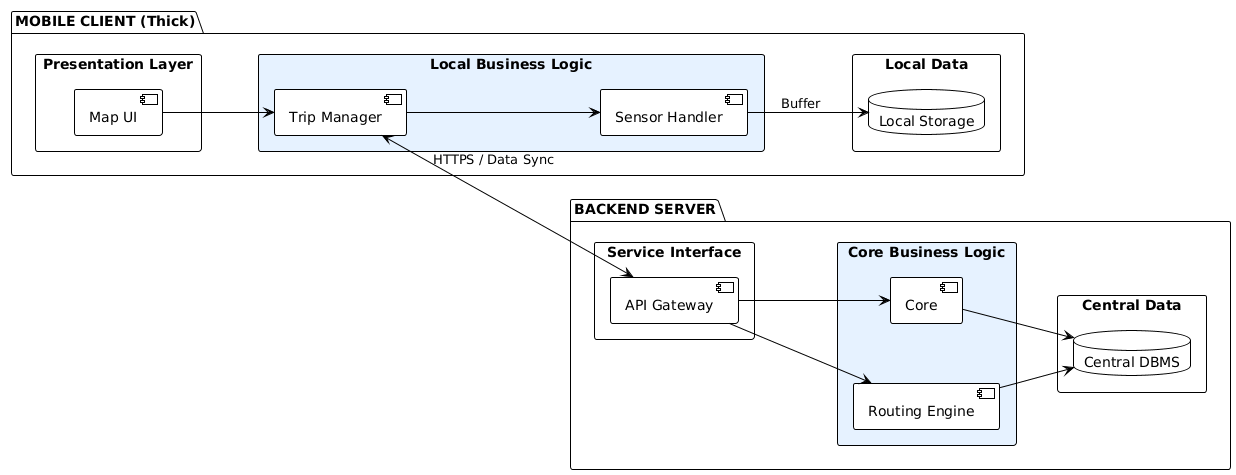
\includegraphics[width=1\textwidth]{DD/img/section2/arc.png} 
    \caption{Thick Client and Fat Server.}
    \label{fig:Client-Server}
\end{figure}


\paragraph{Layered Architecture}
The system is logically structured into three fundamental layers, distributed across the various nodes:


\begin{itemize}
    \item \textbf{Presentation Layer:} Resides entirely on the Mobile Client. It is responsible for all user interactions, the rendering of map tiles, and the visualization of statistical graphs. It also handles tactile input for the verification of automatically detected anomalies \textbf{[G6]}.
    
    \item \textbf{Application Logic Layer:} This layer is distributed.
    \begin{itemize}
        \item \textit{Client-Side:} manages the polling of hardware sensors, the algorithm for pothole detection, the lifecycle of trip recording, and the synchronization of local buffers.
        \item \textit{Server-Side:} manages authentication, validation of incoming data packets, integration with external Weather APIs \textbf{[G3]}, and the core pathfinding algorithms \textbf{[G8]}.
    \end{itemize}
    
    \item \textbf{Data Layer:} Manages the secure storage and retrieval of information. It consists of a Central DBMS (on the server) acting as the single source of truth for public data and user accounts, and a Local Storage (on the client) acting as a temporary buffer and cache to guarantee offline availability \textbf{[SSA3]}.
\end{itemize}

\begin{figure}[H]
    \centering
    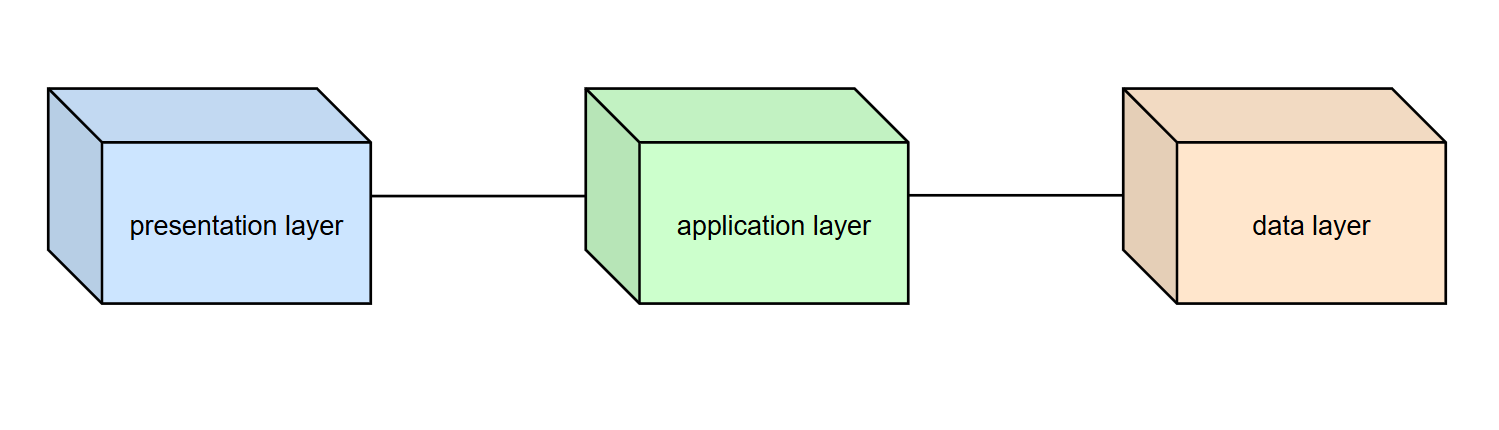
\includegraphics[width=1\textwidth]{DD/img/section2/Layers.png} 
    \caption{Three Layers Application}
    \label{fig:three_layers}
\end{figure}

\paragraph{Physical Tiers}
The logical architecture described above is deployed physically across distinct Tiers (processing nodes):

\begin{itemize}
    \item \textbf{Tier 1 (Client Tier):} Composed of the users' mobile devices (Smartphones). It executes the BBP mobile application and communicates via secure HTTPS protocol.
    
    \item \textbf{Tier 2 (Application Tier):} Composed of the servers hosting the BBP backend logic. This tier exposes the RESTful APIs consumed by the client. To ensure reliability \textbf{[SSA4]} and scalability \textbf{[PR5]}, this tier typically includes Load Balancers to distribute traffic among multiple server instances.
    
    \item \textbf{Tier 3 (Data Tier):} Composed of servers dedicated to the Database Management System (DBMS). This tier is isolated for security and performance reasons and is accessible only by Tier 2.
    
    \item \textbf{External Tier:} Includes third-party services essential for system operation, specifically Map Providers (e.g., Google Maps/OpenStreetMap) and Weather Services (e.g., OpenWeatherMap), integrated via dedicated API interfaces.
\end{itemize}

\begin{figure}[H]
    \centering
    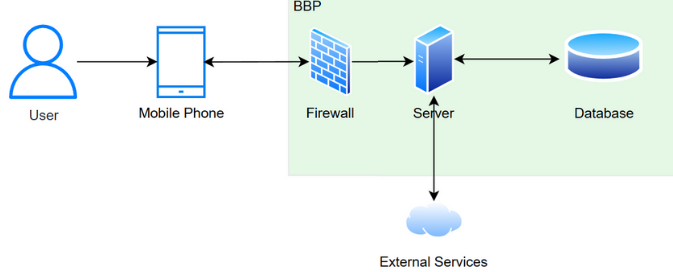
\includegraphics[width=1\textwidth]{DD/img/section2/Architecture.png} 
    \caption{Architecture of the application}
    \label{fig:Architecture}
\end{figure}

\clearpage
\subsection{Component view}
Figure \ref{fig:component_diagram} illustrates the internal decomposition of the system into logical modules and their dependencies. The architecture is split between the Mobile Client, responsible for real-time data acquisition, and the Backend Server, responsible for data aggregation and heavy lifting.

\begin{figure}[H]
    \centering
    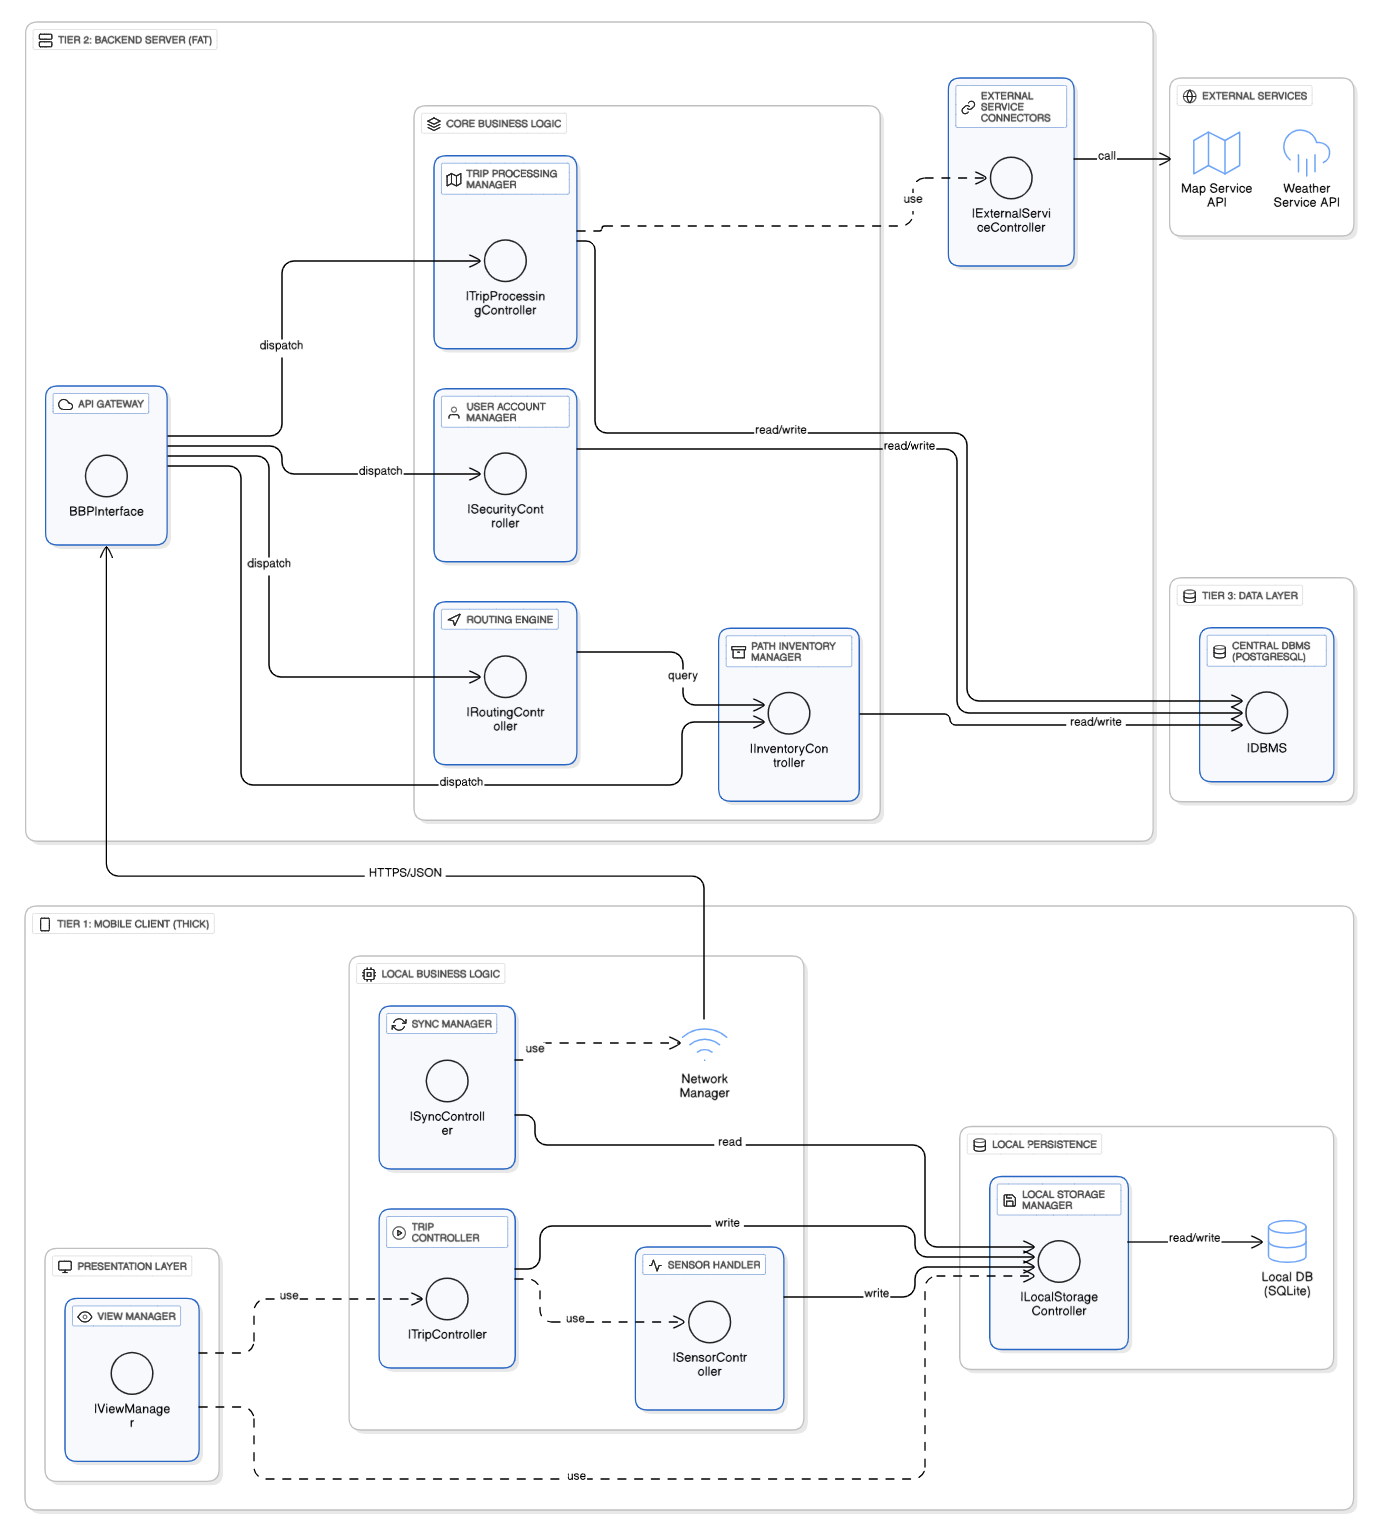
\includegraphics[width=\textwidth]{DD/img/section2/component_view.png}
    \caption{High-level Component Diagram of BBP System}
    \label{fig:component_diagram}
\end{figure}
\clearpage

\paragraph{BBP Mobile Application Components (Client-Side)}
As a ``Thick Client'', the mobile application hosts significant business logic to ensure responsiveness and offline capabilities [CON3].

\begin{itemize}
    \item \textbf{View Manager (UI Layer)}: This component handles the rendering of the user interface. It manages the dashboard, the map visualization (integrating map tiles from the external provider), and user interaction flows. It implements the Model-View-Controller (MVC) pattern to separate presentation from logic.

    \item \textbf{Sensor Handler}: A critical module responsible for interacting with the device hardware. It performs continuous polling of the \textit{Accelerometer}, \textit{Gyroscope}, and \textit{GPS} at high frequency (50Hz) [PR3]. It implements local filtering algorithms to distinguish between user movements (e.g., pedaling) and road anomalies (e.g., potholes), reducing false positives before storage.

    \item \textbf{Trip Controller}: This component manages the lifecycle of a cycling session (Start, Pause, Stop). It orchestrates the flow of data between the \textit{Sensor Handler} and the \textit{Local Storage Manager}, ensuring recording continues seamlessly in the background.

    \item \textbf{Local Storage Manager}: Acts as the interface for the local database (e.g., SQLite). It handles the persistence of raw sensor data, temporary trip logs, and cached map data, ensuring data integrity in case of unexpected application termination.

    \item \textbf{Sync Manager}: Responsible for data synchronization. It monitors connectivity status and, when available, uploads pending trips/anomalies to the backend while downloading updates for the local cache.

    \item \textbf{Network Manager}: Handles all HTTP/HTTPS communications, managing API request headers, token authentication (JWT), and response parsing.
\end{itemize}
\clearpage

\paragraph{BBP Backend Server Components (Server-Side)}
The backend server acts as the centralized authority for data aggregation and user management.

\begin{itemize}
    \item \textbf{API Gateway}: The single entry point for all client requests. It handles routing, rate limiting, and validates authentication tokens before forwarding requests to internal managers.

    \item \textbf{User Account Manager}: Manages user identities, registration, and login processes. It interacts with the DBMS to store credentials securely.

    \item \textbf{Trip Processing Manager}: Receives raw trip data, performs post-processing, calculates final statistics, and invokes the \textit{Weather Connector} to enrich trips with meteorological data [G3].

    \item \textbf{Path Inventory Manager}: The core component for the collaborative map. It stores confirmed anomalies, manages data visibility (Private vs. Public), and executes anonymization routines to strip personal identifiers from published data [G11].

    \item \textbf{Routing Engine}: Calculates optimal bike paths based on user queries. It weights graph edges using the \textbf{Path Score} derived from the \textit{Path Inventory Manager}, prioritizing safety and maintenance over distance [G9].

    \item \textbf{External Service Connectors}: Adapters that communicate with external APIs (Weather Service for conditions, Map Service for topology).
\end{itemize}
\clearpage

\subsection{Deployment view}

\begin{figure}[H]
    \centering
    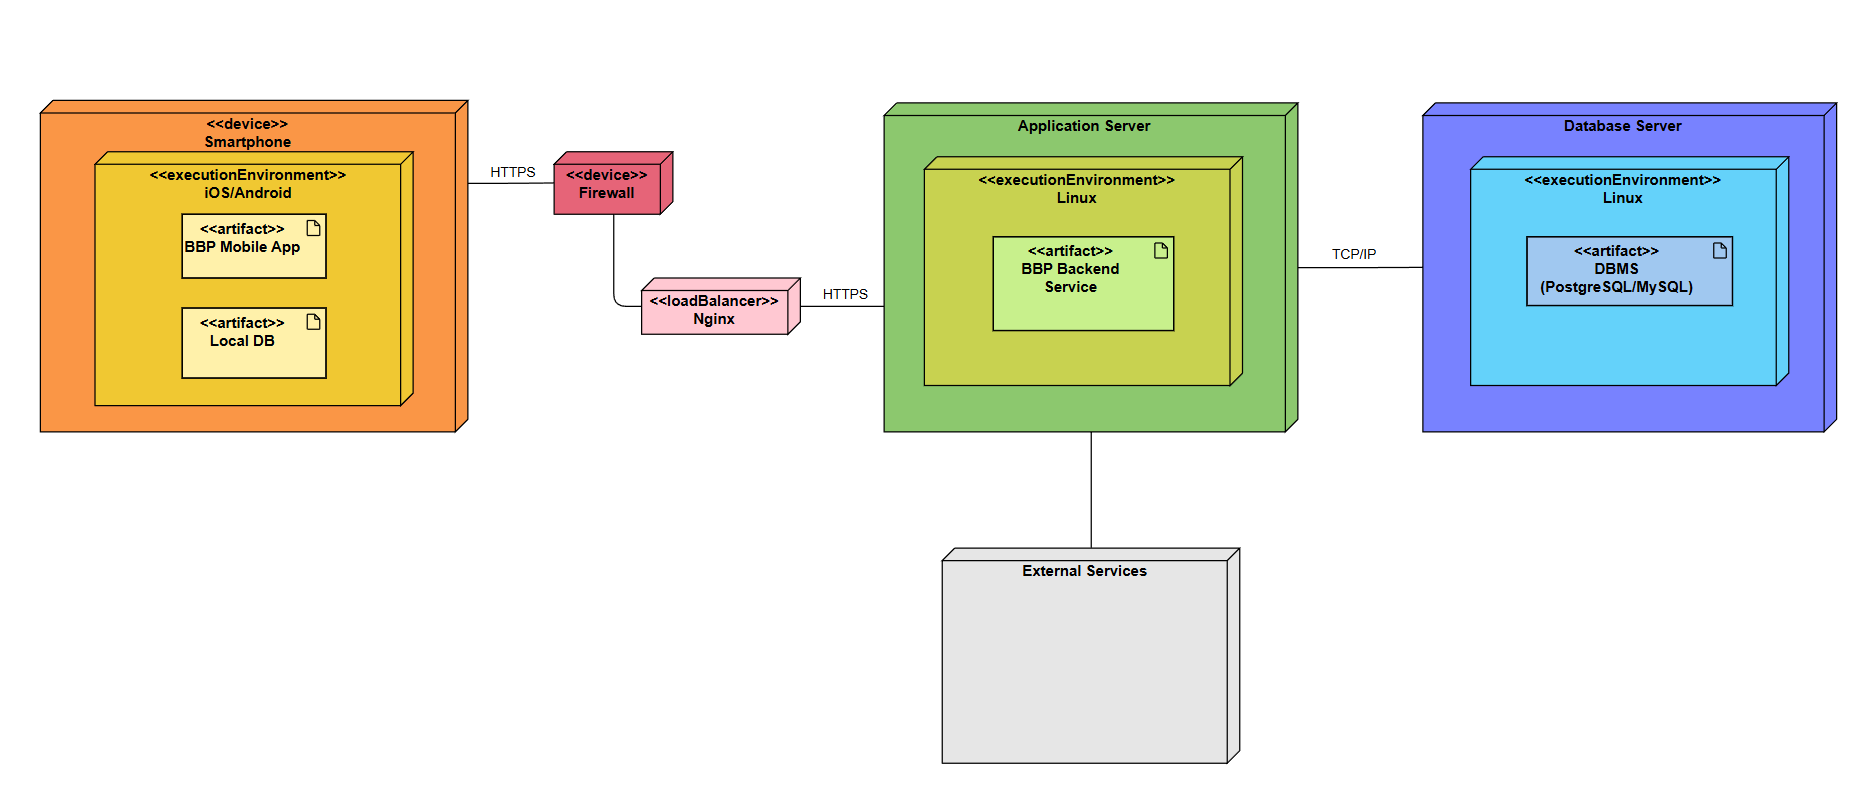
\includegraphics[width=\textwidth]{DD/img/section2/Deployment View.png} 
    \caption{Deployment Diagram}
    \label{fig:deployment_diagram}
\end{figure}

The deployment diagram in Figure \ref{fig:deployment_diagram} shows the hardware components needed for correct system behavior and the protocols used for communication.
As shown in the image, the architecture includes infrastructure elements such as Firewalls and Load Balancers to manage the data stream from user devices to the backend servers.

First of all, \textbf{Firewalls} are in charge of filtering packets received from the Internet to ensure network security. Then, the packets pass through the \textbf{Load Balancer}, where the workload is distributed among the available server instances to increase capacity, reliability, and fault tolerance \textbf{[SSA4]}.

Each device has its own Operating System where the software runs. The tiers represented in the diagram are the following:

\begin{itemize}
    \item \textbf{Tier 1 (Client Device):} It is the client machine, specifically the users' smartphones (Android or iOS). It executes the BBP Mobile Application (Thick Client). Unlike a traditional web client, this tier utilizes local hardware resources not only for presentation but also for:
    \begin{itemize}
        \item \textbf{Processing:} executing the anomaly detection algorithms on raw sensor data.
        \item \textbf{Storage:} managing the Local Database (SQLite/Realm) to buffer trip data when offline connectivity is detected \textbf{[CON3]}.
    \end{itemize}

    \item \textbf{Tier 2 (Application Server):} It contains the application servers, which run the core functionalities of the BBP system. The entire server-side application logic (described in Section 2.2) is mapped into this tier.
    It communicates with the Client Tier through secure RESTful APIs (HTTPS/JSON). Ideally, this tier is composed of a cluster of replicated servers to guarantee scalability \textbf{ [PR5]}. It acts as the orchestrator, processing requests, calculating path scores, and interacting with external services.

    \item \textbf{Tier 3 (Data Server):} It is composed of servers dedicated to the Database Management System (DBMS). They store persistent data (User profiles, Trip History, Public Path Inventory) and execute queries according to the instructions given by the Application Servers. To ensure performance, this tier is physically separated from the application logic.

    \item \textbf{External Services:} While not a tier under the direct control of the BBP system, this node represents the third-party providers (Map Service and Weather Service) that the Application Server contacts via specific APIs to enrich trip data and perform geocoding tasks.
\end{itemize}
\clearpage

\subsection{Runtime View}
\noindent \textbf{Note on Infrastructure Transparency:} \\
For the sake of clarity and readability in the following sequence diagrams, the \textit{Load Balancer} infrastructure layer (previously detailed in the Deployment View, Section 2.C) has been omitted from the lifelines. It is implied that all incoming HTTP/HTTPS traffic directed to the \texttt{API Gateway} physically passes through the Load Balancer first, which handles SSL termination and traffic distribution among available server instances.
\subsubsection{User Registration}
This runtime view illustrates the onboarding process for a new user. The flow initiates in the View Manager, which collects the user's personal details (username, email, password). These are passed to the Network Manager, which handles the secure transmission to the API Gateway on the server. The request is routed to the User Manager, which queries the Central DBMS to verify that the email is not already in use. Upon successful validation, the manager creates a new user record in the database, completing the registration phase.
\begin{figure}[H]
    \centering
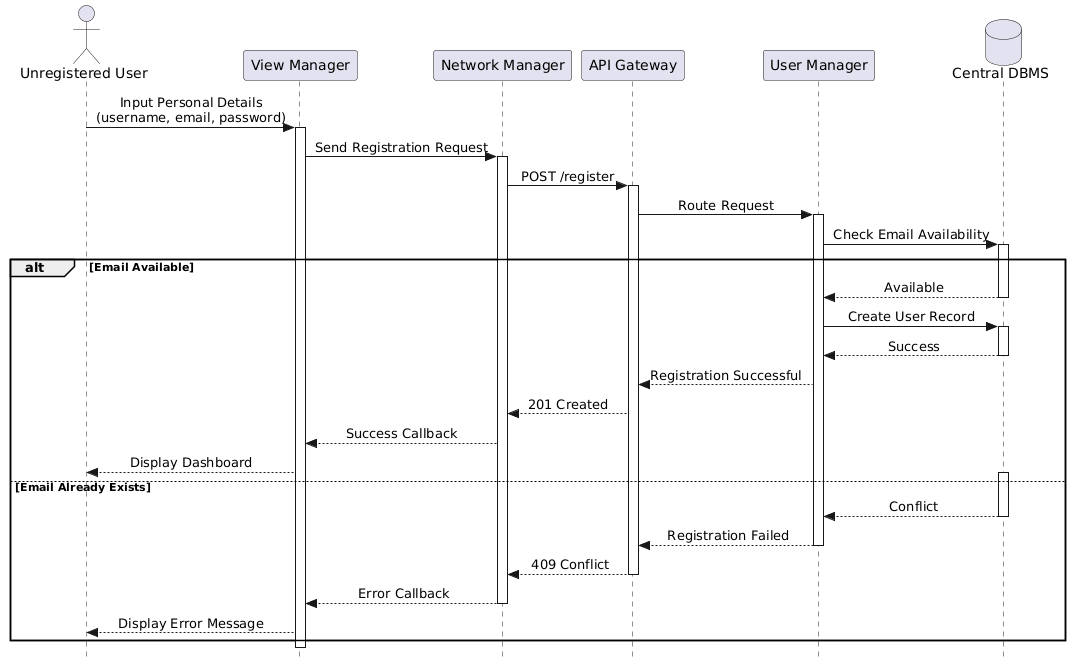
\includegraphics[width=\textwidth]{DD/img/section2/rv/rv1.png} 
    \caption{User Registration}
\end{figure}
\clearpage

\subsubsection{User Login}
This sequence describes the establishment of a secure session. The user enters credentials via the View Manager, which are transmitted by the Network Manager to the backend. The User Account Manager authenticates the credentials against the Central DBMS. If valid, the server generates a secure session token (JWT) and returns it to the client. The diagram highlights the critical role of the Local Storage Manager in securely caching this token on the device, ensuring session persistence and eliminating the need for constant re-authentication.
\begin{figure}[H]
    \centering
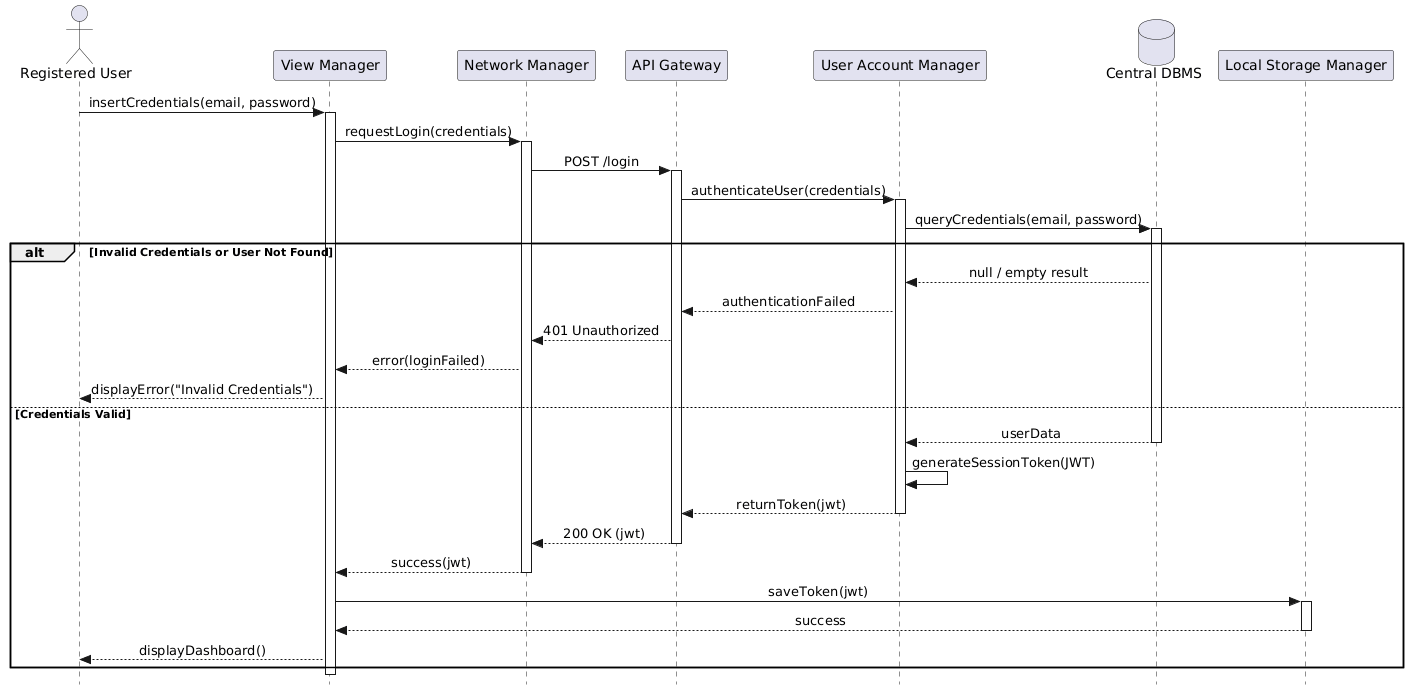
\includegraphics[width=\textwidth]{DD/img/section2/rv/rv2.png} 
    \caption{User Login}
\end{figure}
\clearpage

\subsubsection{Route Planning and Scoring}
This sequence describes the interaction required to generate an optimized cycling route. The process is triggered by a query in the View Manager, which is forwarded via API to the Routing Engine on the backend. This view is critical as it demonstrates the server-side aggregation logic: the Routing Engine must simultaneously retrieve topological data from the External Map Service and quality metrics from the Path Inventory Manager (visualized as Inventory Manager). The diagram details how these sources are synthesized to calculate the ``Path Score,'' returning a ranked list of routes to the client.
\begin{figure}[H]
    \centering
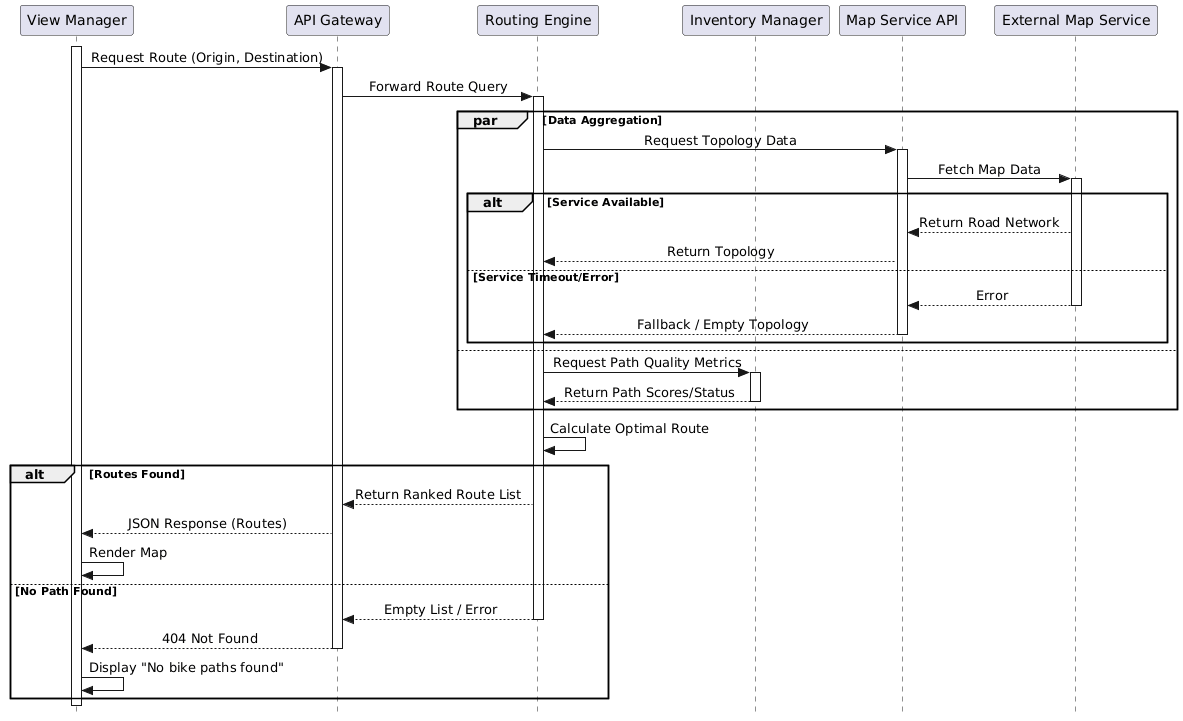
\includegraphics[width=\textwidth]{DD/img/section2/rv/rv3.png} 
    \caption{Route Planning and Scoring}
\end{figure}
\clearpage

\subsubsection{User Login}
This view depicts the core "Thick Client" logic, emphasizing the system's ability to function without network connectivity. The sequence is orchestrated locally by the Trip Manager, which initializes the session. The diagram focuses on the high-frequency interaction between the Sensor Handler and the hardware sensors, showing how raw telemetry is filtered in real-time. Crucially, it illustrates the exclusive reliance on the Local Storage Manager during the active trip, ensuring that all data is buffered to the internal SQLite database to prevent data loss.
\begin{figure}[H]
    \centering
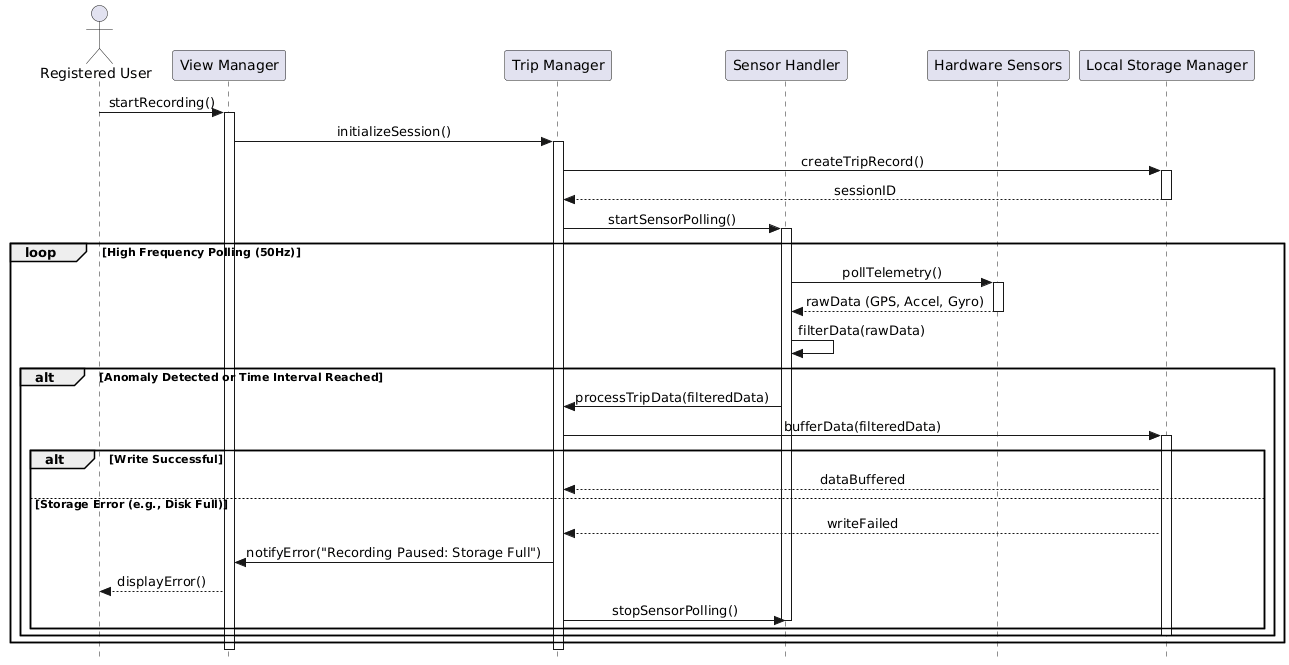
\includegraphics[width=\textwidth]{DD/img/section2/rv/rv4.png} 
    \caption{User Login}
\end{figure}
\clearpage

\subsubsection{Data Synchronization and Upload}
This runtime view details the "handover" mechanism that moves data from the local buffer to the central system once connectivity is restored. The sequence is initiated by the Sync Manager, which monitors network status in the background. The diagram shows the Sync Manager retrieving pending trips from Local Storage and batching them to the API Gateway. It further illustrates the server-side acknowledgment from the Trip Manager, allowing the client to safely flag the local records as "Synced" and free up storage space.
\begin{figure}[H]
    \centering
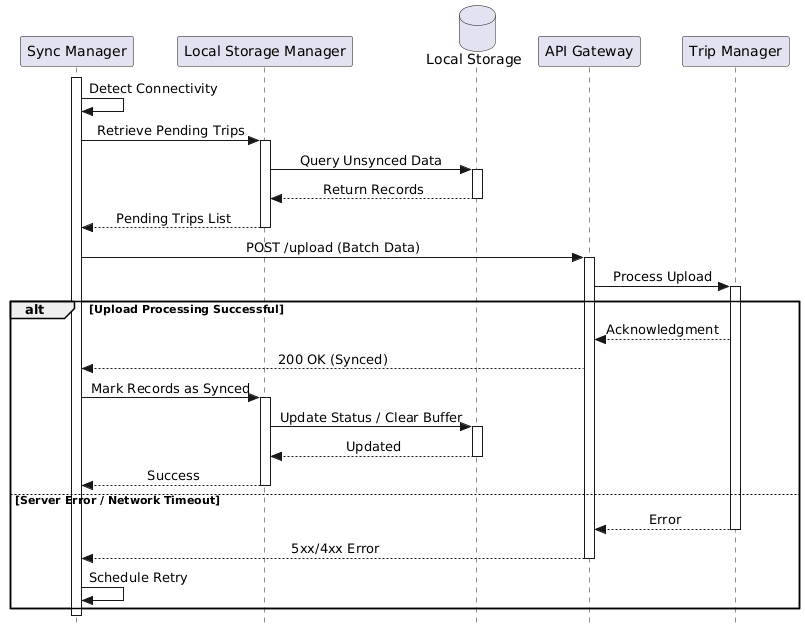
\includegraphics[width=\textwidth]{DD/img/section2/rv/rv5.png} 
    \caption{Data Synchronization and Upload}
\end{figure}
\clearpage

\subsubsection{Post-Trip Data Enrichment}
This sequence describes the server-side data processing that occurs immediately after a trip upload. The interaction is driven by the Trip Manager, which parses the uploaded geospatial data. The view highlights the integration with the Weather Connector, showing how specific timestamps and coordinates are used to query the External Weather Service API. The sequence concludes with the merging of this contextual meteorological data into the trip record and its final persistence in the Central DBMS, ensuring that statistical reports are rich and accurate.
\begin{figure}[H]
    \centering
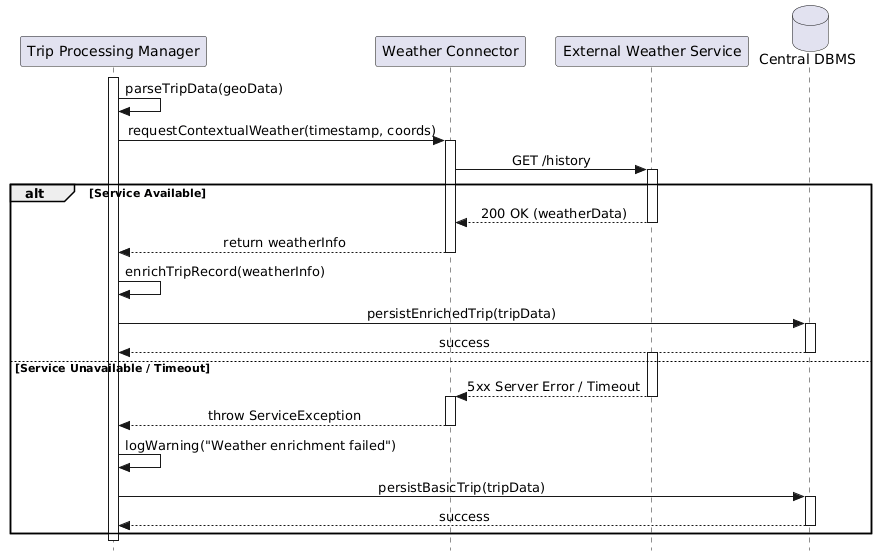
\includegraphics[width=\textwidth]{DD/img/section2/rv/rv6.png} 
    \caption{Post-Trip Data Enrichment}
\end{figure}
\clearpage

\subsubsection{Anomaly Verification and Confirmation}
This view outlines the collaborative verification process, which transforms automated sensor flags into confirmed community data. The sequence begins with the View Manager presenting "Suspected Anomalies" retrieved from Local Storage to the user. The diagram traces the flow of a user's confirmation action (Confirm/Reject) through the Sync Manager to the backend. It specifically highlights the role of the Path Inventory Manager in receiving this validation and updating the status of the anomaly in the Central DBMS from a tentative flag to a verified obstacle.
\begin{figure}[H]
    \centering
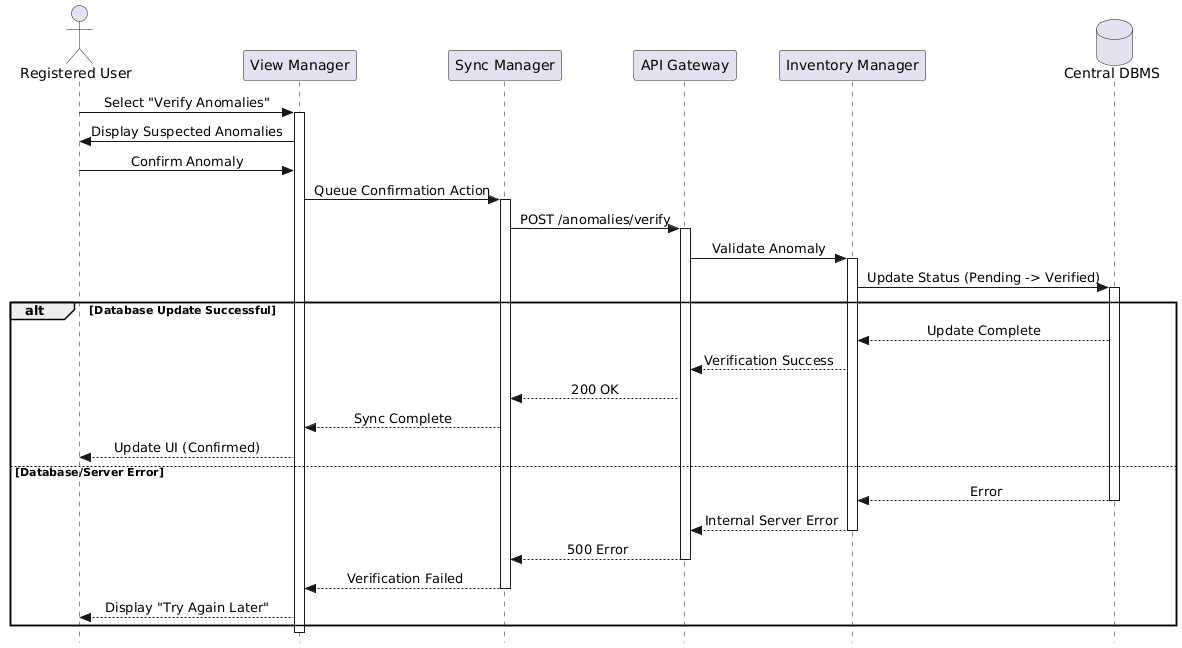
\includegraphics[width=\textwidth]{DD/img/section2/rv/rv7.png} 
    \caption{Anomaly Verification and Confirmation}
\end{figure}
\clearpage

\subsubsection{Data Publication and Anonymization}
This runtime view addresses the privacy constraints required when sharing personal data with the public inventory. The sequence is triggered when a user selects a private trip for publication. The diagram focuses on the Path Inventory Manager executing the anonymization routine, explicitly showing the removal of the User ID and the truncation of start/end coordinates before the data is committed to the Public Inventory. It concludes with the Routing Engine being triggered to recalculate path scores based on this newly available public data.
\begin{figure}[H]
    \centering
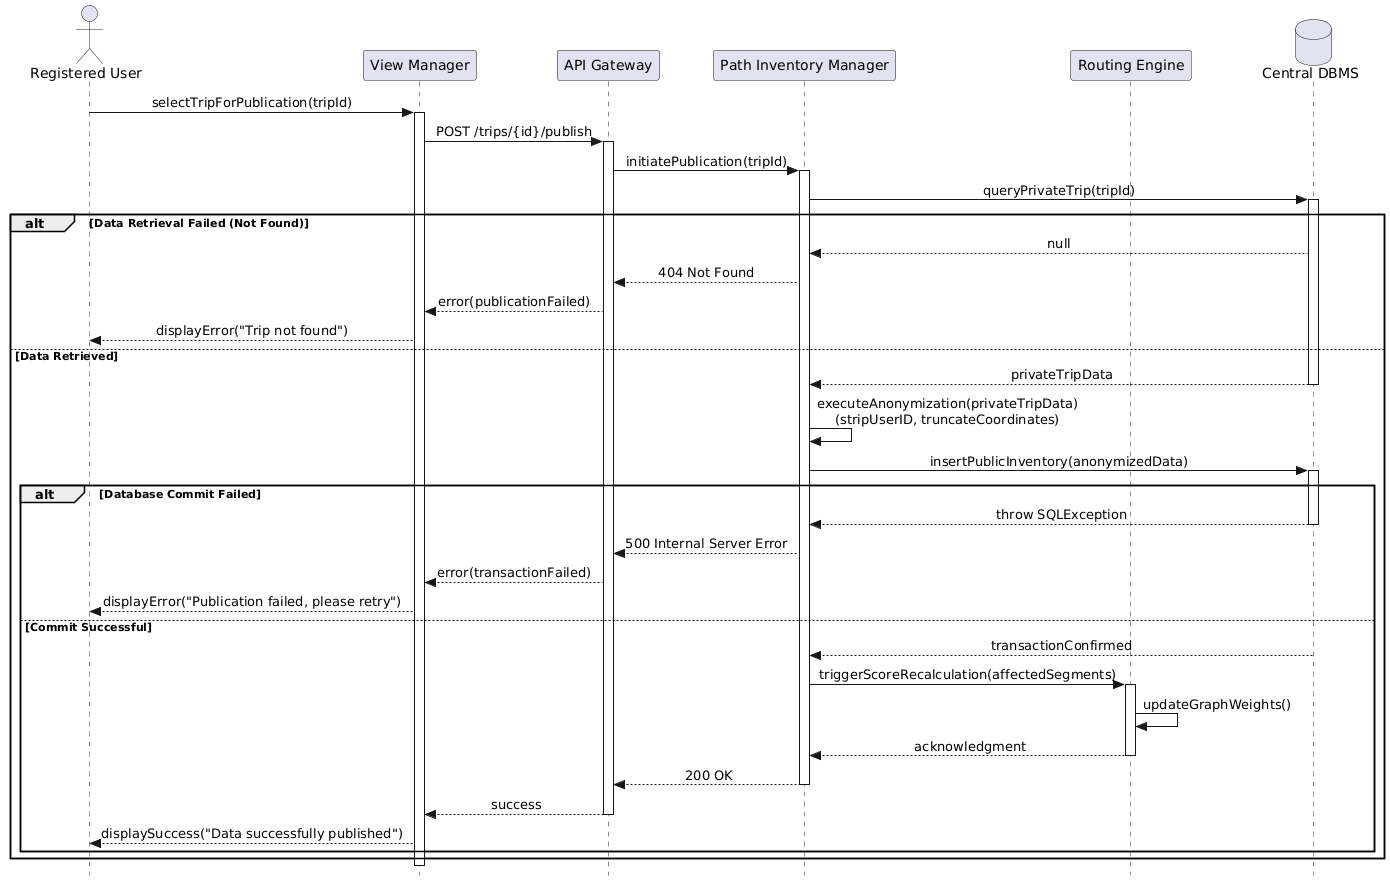
\includegraphics[width=\textwidth]{DD/img/section2/rv/rv8.png} 
    \caption{Anomaly Verification and Confirmation}
\end{figure}
\clearpage

\subsubsection{Automatic Activity Recognition}
This view demonstrates the background monitoring capability required to detect cycling without user intervention. The sequence shows the Sensor Handler operating in a low-power mode (to adhere to battery constraints), periodically sampling the accelerometer. The diagram illustrates the transition from passive monitoring to active recording: upon detecting a specific speed threshold, the Sensor Handler wakes the Trip Controller, which instantiates a new session in Local Storage and issues a notification to the user.
\begin{figure}[H]
    \centering
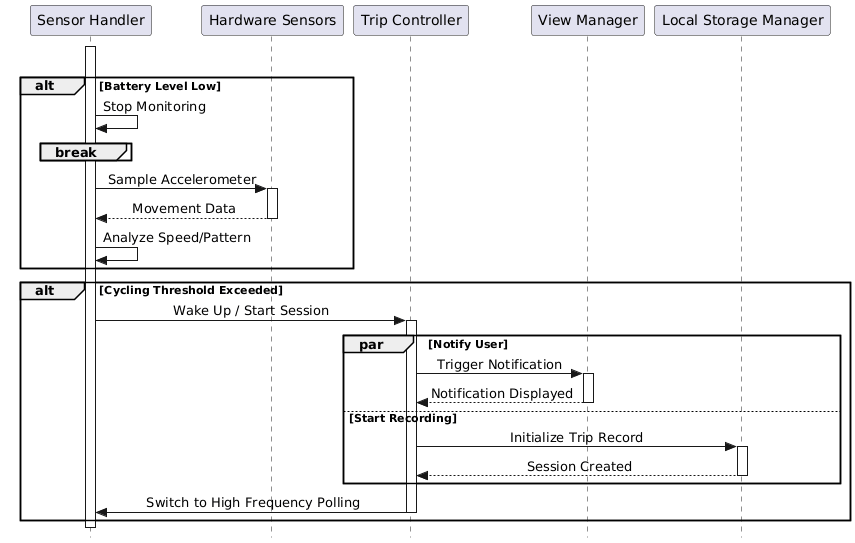
\includegraphics[width=\textwidth]{DD/img/section2/rv/rv9.png} 
    \caption{Automatic Activity Recognition}
\end{figure}
\clearpage

\subsubsection{Manual Path Reporting}
This sequence details the flow for user-initiated reports regarding path conditions. The interaction begins in the View Manager, where the user selects a map location. The diagram emphasizes the "Offline-First" design: the Trip Controller first saves the report object via the Local Storage Manager, ensuring instantaneous user feedback. The Sync Manager is then shown detecting this new pending object and transmitting it to the Path Inventory Manager on the server for validation and storage in the Central DBMS.
\begin{figure}[H]
    \centering
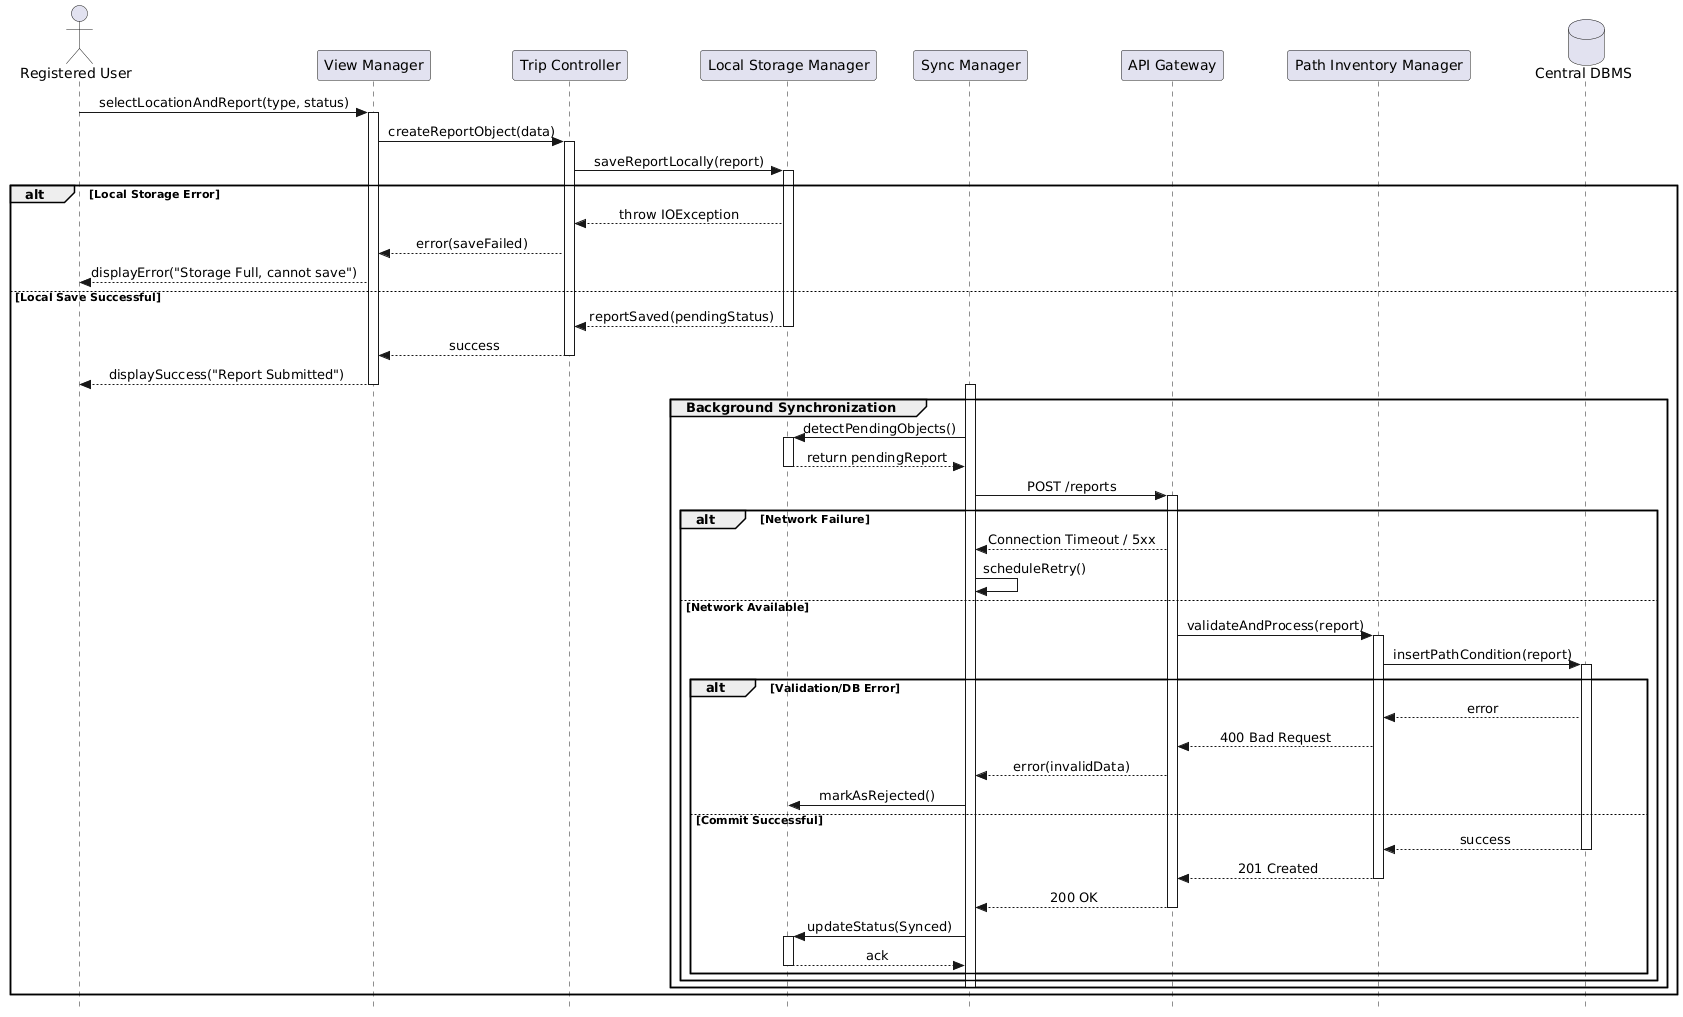
\includegraphics[width=\textwidth]{DD/img/section2/rv/rv10.png} 
    \caption {Manual Path Reporting}
\end{figure}
\clearpage

\subsubsection{History Retrieval and Visualization}
This view describes the data retrieval process for viewing past activities, showcasing the hybrid data loading strategy. The sequence is initiated when the user accesses the history screen. The diagram illustrates parallel retrieval: the View Manager immediately renders cached summaries from Local Storage for instant feedback, while the Sync Manager simultaneously queries the API Gateway for any updates. The flow concludes with the Sync Manager updating the local database with data received from the server, ensuring consistency between the two sources.
\begin{figure}[H]
    \centering
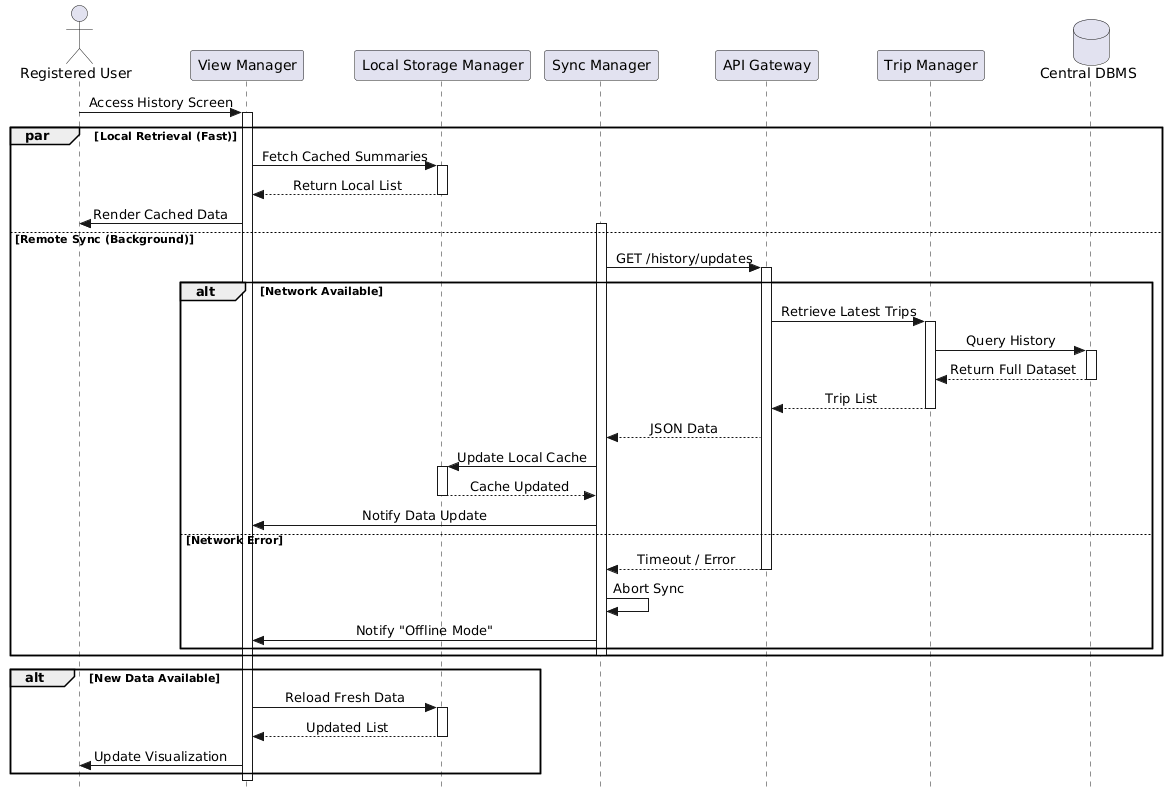
\includegraphics[width=\textwidth]{DD/img/section2/rv/rv11.png} 
    \caption{History Retrieval and Visualization}
\end{figure}
\clearpage

\subsection{Component Interfaces}
This section details the interfaces exposed by the system components. Following the architecture defined in Section 2.2, we distinguish between \textbf{External Interfaces} (boundaries between the Mobile App and the Backend) and \textbf{Internal Controllers} (interfaces used for inter-component communication within the Mobile Client and the Backend Server).

\subsubsection{Mobile Client Interfaces (Tier 1)}
As the Mobile Application acts as a \textbf{Thick Client}, it contains significant business logic. The following interfaces manage the local orchestration of sensors, storage, and synchronization.
\begin{figure}[H]
    \centering
    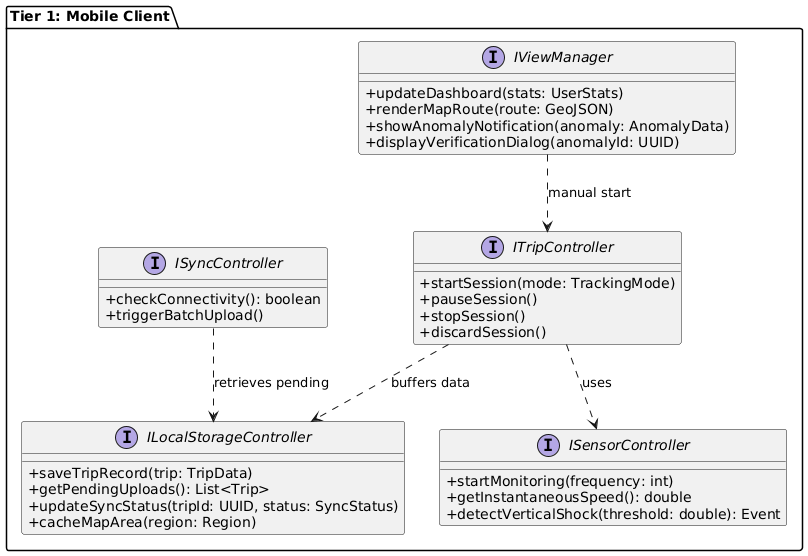
\includegraphics[width=\textwidth]{DD/img/section2/ifs/if1.png}
    \caption{Mobile Client Interfaces}
\end{figure}

\begin{itemize}
    \item \begin{minipage}[t]{\linewidth}
        \textbf{\texttt{ViewManagerInterface}}
        \begin{itemize}
            \item \textbf{Description:} The boundary interface between the User Interface (UI) views and the application logic. It allows the logic layers to push updates to the user.
            \item \textbf{Methods:}
            \begin{itemize}
                \item \texttt{updateDashboard(stats: UserStats)}: Updates total distance and average speed on the home screen.
                \item \texttt{renderMapRoute(route: GeoJSON)}: Draws the calculated path on the map view.
                \item \texttt{showAnomalyNotification(anomaly: AnomalyData)}: Triggers the push notification for detected obstacles.
                \item \texttt{displayVerificationDialog(anomalyId: UUID)}: Opens the popup for the user to confirm/reject a pothole.
            \end{itemize}
        \end{itemize}
    \end{minipage}

    \item \begin{minipage}[t]{\linewidth}
        \textbf{\texttt{TripController}}
        \begin{itemize}
            \item \textbf{Description:} Internal interface exposed by the \textbf{Trip Manager} component. It acts as the state machine for the cycling session.
            \item \textbf{Used By:} \texttt{ViewManager} (Manual Start), \texttt{SensorHandler} (Auto-Start).
            \item \textbf{Methods:}
            \begin{itemize}
                \item \texttt{startSession(mode: TrackingMode)}: Initializes a new trip (Manual or Automated).
                \item \texttt{pauseSession()}: Temporarily halts recording.
                \item \texttt{stopSession()}: Finalizes the trip and triggers the local save.
                \item \texttt{discardSession()}: Deletes current temporary data without saving.
            \end{itemize}
        \end{itemize}
    \end{minipage}

    \item \begin{minipage}[t]{\linewidth}
        \textbf{\texttt{SensorController}}
        \begin{itemize}
            \item \textbf{Description:} Internal interface exposed by the \textbf{Sensor Handler}. It abstracts the low-level hardware access (GPS, Accelerometer, Gyroscope).
            \item \textbf{Used By:} \texttt{TripController}.
            \item \textbf{Methods:}
            \begin{itemize}
                \item \texttt{startMonitoring(frequency: int)}: Activates sensors at high frequency (50Hz) for anomaly detection.
                \item \texttt{getInstantaneousSpeed(): double}: Returns current speed for Automatic Activity Recognition.
                \item \texttt{detectVerticalShock(threshold: double): Event}: Returns an event if accelerometer Z-axis variance exceeds the threshold (pothole detection).
            \end{itemize}
        \end{itemize}
    \end{minipage}

    \item \begin{minipage}[t]{\linewidth}
        \textbf{\texttt{LocalStorageController}}
        \begin{itemize}
            \item \textbf{Description:} Internal interface exposed by the \textbf{Local Storage Manager}. It manages persistence on the device (SQLite/Realm).
            \item \textbf{Used By:} \texttt{TripController}, \texttt{SyncManager}.
            \item \textbf{Methods:}
            \begin{itemize}
                \item \texttt{saveTripRecord(trip: TripData)}: Buffers the trip data locally when offline.
                \item \texttt{getPendingUploads(): List<Trip>}: Retrieves trips that have not yet been synced to the server.
                \item \texttt{updateSyncStatus(tripId: UUID, status: SyncStatus)}: Marks a record as "Uploaded" after successful sync.
                \item \texttt{cacheMapArea(region: Region)}: Stores map tiles for offline usage.
            \end{itemize}
        \end{itemize}
    \end{minipage}

    \item \begin{minipage}[t]{\linewidth}
        \textbf{\texttt{SyncController}}
        \begin{itemize}
            \item \textbf{Description:} Internal interface exposed by the \textbf{Sync Manager}. It handles the data handover logic.
            \item \textbf{Used By:} \texttt{NetworkManager}.
            \item \textbf{Methods:}
            \begin{itemize}
                \item \texttt{checkConnectivity(): boolean}: Verifies if the backend is reachable.
                \item \texttt{triggerBatchUpload()}: Initiates the upload of all pending trips.
            \end{itemize}
        \end{itemize}
    \end{minipage}
\end{itemize}
\clearpage

\subsubsection{Backend Server Interfaces (Tier 2)}
The Backend Server exposes a public REST API via the Gateway and uses internal Controllers to manage the complex business logic (Scoring, Anonymization, Aggregation).
\begin{figure}[H]
    \centering
    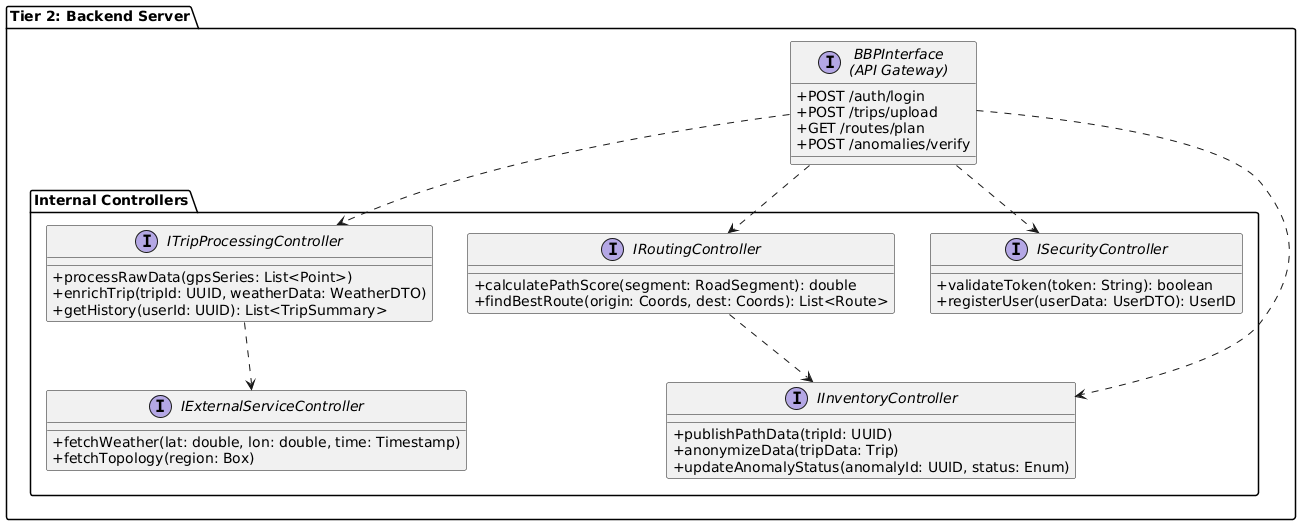
\includegraphics[width=\textwidth]{DD/img/section2/ifs/if2.png}
    \caption{Backend Server Interfaces}
\end{figure}


\paragraph{External Interfaces (REST API)}
\begin{itemize}
    \item \begin{minipage}[t]{\linewidth}
        \textbf{\texttt{BBPInterface}} (API Gateway)
        \begin{itemize}
            \item \textbf{Description:} The main entry point for the Mobile Client. It routes incoming HTTP requests to the appropriate internal controller.
            \item \textbf{Methods:}
            \begin{itemize}
                \item \texttt{POST /auth/login}: Handles credential verification.
                \item \texttt{POST /trips/upload}: Receives raw trip data (GPS + Anomalies) from the client.
                \item \texttt{GET /routes/plan}: Accepts origin/destination and returns ranked routes.
                \item \texttt{POST /anomalies/verify}: Accepts user confirmation of detected obstacles.
            \end{itemize}
        \end{itemize}
    \end{minipage}
\end{itemize}
\clearpage

\paragraph{Internal Controllers (Server Logic)}
\begin{itemize}
    \item \begin{minipage}[t]{\linewidth}
        \textbf{\texttt{SecurityController}}
        \begin{itemize}
            \item \textbf{Description:} Interface exposed by the \textbf{User Account Manager}. It handles authentication and token management.
            \item \textbf{Methods:}
            \begin{itemize}
                \item \texttt{validateToken(token: String): boolean}: Checks the validity of the JWT for every incoming request.
                \item \texttt{registerUser(userData: UserDTO): UserID}: Creates a new user record in the DBMS.
            \end{itemize}
        \end{itemize}
    \end{minipage}

    \item \begin{minipage}[t]{\linewidth}
        \textbf{\texttt{TripProcessingController}}
        \begin{itemize}
            \item \textbf{Description:} Interface exposed by the \textbf{Trip Processing Manager}. It handles post-processing of raw data.
            \item \textbf{Methods:}
            \begin{itemize}
                \item \texttt{processRawData(gpsSeries: List<Point>)}: Cleans GPS noise and calculates average speed/distance.
                \item \texttt{enrichTripRecord(tripId: UUID, weatherData: WeatherDTO)}: Merges trip statistics with meteorological data.
                \item \texttt{getHistory(userId: UUID): List<TripSummary>}: Retrieves past trips for the history view.
            \end{itemize}
        \end{itemize}
    \end{minipage}

    \item \begin{minipage}[t]{\linewidth}
        \textbf{\texttt{InventoryController}}
        \begin{itemize}
            \item \textbf{Description:} Interface exposed by the \textbf{Path Inventory Manager}. It manages the shared knowledge base.
            \item \textbf{Methods:}
            \begin{itemize}
                \item \texttt{publishPathData(tripId: UUID)}: Changes visibility from Private to Public.
                \item \texttt{anonymizeData(tripData: Trip)}: Strips user IDs and truncates start/end coordinates before publication.
                \item \texttt{updateAnomalyStatus(anomalyId: UUID, status: Verified|Rejected)}: Updates the reliability of a reported obstacle.
            \end{itemize}
        \end{itemize}
    \end{minipage}

    \item \begin{minipage}[t]{\linewidth}
        \textbf{\texttt{RoutingController}}
        \begin{itemize}
            \item \textbf{Description:} Interface exposed by the \textbf{Routing Engine}. It executes the pathfinding algorithms.
            \item \textbf{Methods:}
            \begin{itemize}
                \item \texttt{calculatePathScore(segment: RoadSegment): double}: Computes the score based on surface quality and obstacles.
                \item \texttt{findBestRoute(origin: Coords, dest: Coords): List<Route>}: Returns the optimal path prioritizing the Path Score.
            \end{itemize}
        \end{itemize}
    \end{minipage}

    \item \begin{minipage}[t]{\linewidth}
        \textbf{\texttt{ExternalServiceController}}
        \begin{itemize}
            \item \textbf{Description:} Interface exposed by the \textbf{External Service Connectors}. It acts as an adapter/facade for third-party APIs.
            \item \textbf{Methods:}
            \begin{itemize}
                \item \texttt{fetchWeather(lat: double, lon: double, time: Timestamp)}: Contacts the External Weather Service.
                \item \texttt{fetchTopology(region: Box)}: Retrieves road network data from the Map Service Provider.
            \end{itemize}
        \end{itemize}
    \end{minipage}
\end{itemize}
\clearpage

\subsubsection{Data Layer Interfaces (Tier 3)}
\begin{figure}[H]
    \centering
    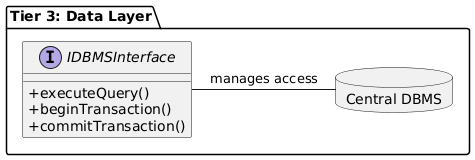
\includegraphics[width=0.6\textwidth]{DD/img/section2/ifs/if3.png}
    \caption{Data Layer Interfaces}
\end{figure}
\begin{itemize}
    \item \begin{minipage}[t]{\linewidth}
        \textbf{\texttt{DBMSInterface}}
        \begin{itemize}
            \item \textbf{Description:} The standard interface used by the Backend Controllers to interact with the Central DBMS.
            \item \textbf{Methods:}
            \begin{itemize}
                \item \texttt{executeQuery()}: Executes read-only queries.
                \item \texttt{beginTransaction()}: Starts a new transaction for data integrity.
                \item \texttt{commitTransaction()}: Commits changes to the database.
            \end{itemize}
        \end{itemize}
    \end{minipage}
\end{itemize}